% 第3章第1节：路径成本与松弛（路径成本与最短路问题；距离标签与松弛）。

\section{路径成本与松弛}
\label{sec:shortest-path-foundations}

不论是只从单一源点出发，还是同时求所有顶点对之间的路线，最短路问题都建立在同一套基础概念之上：先规定怎样度量一条行走的成本、在什么范围内比较长短，再用距离上界标签与逐弧松弛作为推进搜索和核验最优性的共同机制。第~\ref{sec:graph-opt-sp-problem}小节界定路径成本、单源与全源最短路距离以及负环导致的三类结果；第~\ref{sec:graph-opt-sp-relaxation}小节建立距离标签、松弛操作、逐弧三角不等式最优性条件与前驱树恢复。

\subsection{路径成本与最短路问题}
\label{sec:graph-opt-sp-problem}
\label{sec:graph-opt-path-cost}

输入是有限有向图$\mathcal G=(V,E)$，以及每条弧$u\to v$上的一个实数\emph{长度}（或称弧权）$\ell_{u,v}\in\mathbb R$（在全源最短路中亦记作$w(u,v)$）。长度可以表示距离、时间或转换代价，也允许为负，例如某次转换带来收益。候选对象是连接两个顶点的路线，比较的是路线的总成本。对一条从$u=v_0$到$v=v_k$的行走$W=(v_0,v_1,\ldots,v_k)$，规定它的成本为沿途弧长之和：
\begin{equation}
  \ell(W)=\sum_{r=1}^{k}\ell_{v_{r-1},v_r}
  \quad\Bigl(\text{或记作 }w(W)=\sum_{r=1}^{k}w(v_{r-1},v_r)\Bigr).
  \label{eq:graph-opt-walk-cost}
\end{equation}
只含一个顶点的零步行走成本为零。

所有长度都等于$1$时，成本就是边数，回到第~\ref{sec:graph-bfs}节广度优先遍历的情形；一般长度下两者不再一致。例如$s$到$t$有一条长$5$的直达弧，又有经过$u$、两段各长$1$的路线，两步路线反而更短。我们要对关注的顶点对$(u,v)$输出从$u$到$v$的最低成本，以及一条达到这个成本的路线。

“最短路线”还要先说清在哪些路线中比较。一种选择只允许简单路径，即不重复经过顶点的路径；另一种允许一般的行走，顶点和弧都可以重复。有限图中简单路径只有有限条，因此只要终点可达，最小值一定存在；行走可以无限地绕圈，候选有无穷多个，只能谈成本的下确界。

\begin{definition}[最短路距离、单源最短路与全源最短路]
\label{def:graph-opt-shortest-path}
给定有限有向图$\mathcal G=(V,E)$与弧长$\ell_{u,v}\in\mathbb R$（或$w(u,v)\in\mathbb R$）。对任意有序顶点对$(u,v)\in V\times V$，记$\mathcal W_{u,v}$为从$u$到$v$的全部有限行走组成的集合，称
\begin{equation}
  d^*(u,v)=\inf_{W\in\mathcal W_{u,v}}\ell(W)
  \label{eq:graph-opt-shortest-distance}
\end{equation}
为从$u$到$v$的\term{最短路}（shortest path）距离，约定空集的下确界为$+\infty$。若某条行走$W\in\mathcal W_{u,v}$满足$\ell(W)=d^*(u,v)$，就称$W$是一条从$u$到$v$的最短路。
\begin{enumerate}
  \item 固定单一源点$s\in V$，简记$\delta(v)=d^*(s,v)$，求出从$s$到全部顶点$v\in V$的距离$\delta(v)$及相应路线的问题称为\emph{单源最短路}（single-source shortest paths）问题。
  \item 同时求出所有有序顶点对$(u,v)\in V\times V$之间的距离矩阵$\bm D=(d^*(u,v))_{u,v\in V}$及相应路线的问题称为\term{全源最短路}（all-pairs shortest paths, APSP）问题。
\end{enumerate}
\end{definition}

本章的算法计算的都是行走下确界$d^*(u,v)$（单源情形记作$\delta(v)$）。在多数情形中它与简单路径的最小值一致，原因是行走中的绕圈部分可以删掉。

设行走$W$两次经过顶点$x$，两次之间的一段是从$x$回到$x$的闭行走$C$，删去$C$得到更短的行走$W'$，并且
\[
  \ell(W')=\ell(W)-\ell(C).
\]
只要$C$的成本非负，删去它就不会增加成本。反复删除，直到不再有重复顶点，便得到一条成本不超过$\ell(W)$的简单路径。

\paragraph{负环与三类结果}
删除闭合段的论证只在闭合段成本非负时有效。成本为负的有向环称为\term{负环}（negative cycle）。若能从源点$s$走到某个负环，绕若干圈后再走到$v$，则每多绕一圈，成本就再降低一次，于是$\delta(v)=d^*(s,v)=-\infty$。这并不表示存在一条“长度为负无穷的路径”，而是说任何有限成本都能被另一条行走打破。

反过来，若没有这样“从$s$可达、又能到达$v$”的负环，那么$s$到$v$的行走中出现的任一闭合段也不可能为负。原因是一条成本为负的闭行走，在第一个重复顶点处切开，总能分出一个简单环，剩下的部分仍是闭行走。重复这一切分，闭行走的成本就写成若干个简单环的成本之和，其中必有一个为负；这个环位于闭合段上，所以同样从$s$可达、又能到达$v$，与假设矛盾。因此在这种情形下，所有闭合段都可以删除，$\delta(v)$等于简单路径的最小成本，并且由一条简单路径达到。

综上，对任一固定源点$s$，每个顶点$v$的距离属于三类之一：不可达时$\delta(v)=+\infty$；可达且不受负环影响时$\delta(v)$为有限值，并由一条简单路径达到；能从某个$s$可达的负环到达时$\delta(v)=-\infty$。算法的输出也应按这三类给出。

三类顶点可以出现在同一张图中。图~\ref{fig:graph-opt-distance-outcomes}中，负环$a\to b\to a$只影响它自己及其后继$t$；旁支$u$不能从这个负环到达，距离仍是有限的$4$；另一个负环$x\to y\to x$从$s$出发到不了，对本次查询没有任何影响。所以不能因为图中某处有负环，就把全部顶点都标成负无穷。

\begin{figure}[!htb]
  \centering
  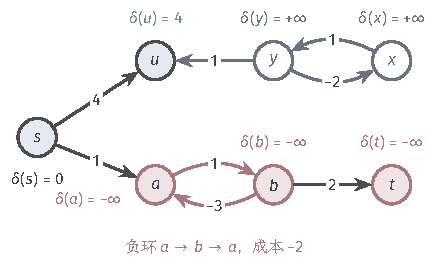
\includegraphics[width=73.801mm]{figures/01-basic-mathematics/04-graphs/tikz/c3-distance-outcomes/figure.pdf}
  \caption{单源最短路的三类结果同处一图（源点为$s$，弧旁数字为长度）。$a\to b\to a$的成本为$1-3=-2$，是从$s$可达的负环，环上的$a,b$及其后继$t$的距离为$-\infty$（红色）；旁支$u$不能从该负环到达，距离为有限值$4$（蓝色）；负环$x\to y\to x$从$s$不可达，$x,y$的距离为$+\infty$（灰色），弧$y\to u$也不会改变$u$的距离。}
  \label{fig:graph-opt-distance-outcomes}
\end{figure}

无向图中的负边需要特别注意。把无向边$\{u,v\}$换成两条同长的反向弧$u\to v$与$v\to u$以后，一条长为负的无向边自己就构成负环：沿它走过去再走回来，成本是两倍的负长度。因此，把含负边的无向图换成有向图后，本章的负环检测算法会将受影响的距离报告为$-\infty$，不能据此求出“只允许简单路径”时的最小值。下文只在无向边长度非负时用这类转换求有限最短路。

\subsection{距离标签与松弛}
\label{sec:graph-opt-sp-relaxation}
\label{sec:graph-opt-relaxation}

最短路算法都不直接枚举行走，而是为每个顶点保存一个当前已知的最好成本，在发现更好的路线时更新它。以固定源点$s$为例，设想已经知道一条从$s$到$u$、成本为$d(u)$的路线，又有弧$u\to v$，那么把这条弧接在路线末尾，就得到一条到$v$、成本为$d(u)+\ell_{u,v}$的路线。如果它比$v$目前记录的成本更低，就应该改用它。

\paragraph{松弛操作}
为每个顶点$v$保存一个\term{距离标签}（distance label）$d(v)\in\mathbb R\cup\{+\infty\}$和一个前驱$p(v)$（在全源最短路中则对每个源点$u$维护一行距离标签$d(u,v)$与前驱$\pi(u,v)$）。单源初始化时令$d(s)=0$，其余顶点$d(v)=+\infty$，前驱为空。对一条弧$u\to v$执行\term{松弛}（relaxation），是指比较当前标签$d(v)$与候选值$d(u)+\ell_{u,v}$：若$d(u)<+\infty$且
\begin{equation}
  d(u)+\ell_{u,v}<d(v),
  \label{eq:graph-opt-relaxation}
\end{equation}
就令$d(v)\leftarrow d(u)+\ell_{u,v}$、$p(v)\leftarrow u$；否则什么也不做。只有严格改善时才更新，因而标签只会下降，不会上升。

图~\ref{fig:graph-opt-relaxation}画出一次松弛的两种结果：候选值$5$小于原标签$8$时，标签与前驱一起改写；原标签已是$4$时，两者都不变。距离数组和前驱数组必须同步修改：如果只改距离而不改前驱，回溯得到的路线成本就不再等于标签。

\begin{figure}[!htb]
  \centering
  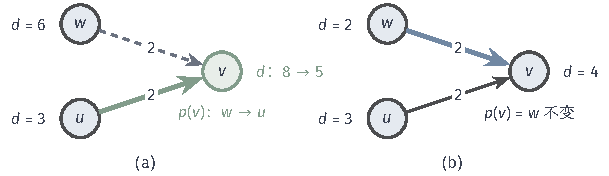
\includegraphics[width=102.993mm]{figures/01-basic-mathematics/04-graphs/tikz/c3-relaxation/figure.pdf}
  \caption{对弧$u\to v$松弛（顶点旁为当前标签，弧旁为长度）。(a) 候选值$d(u)+\ell_{u,v}=3+2=5$小于原标签$8$，标签改为$5$，前驱由$w$改为$u$（绿色表示被改善的标签与新的前驱弧，虚线为被替换的旧前驱弧）。(b) 原标签为$4$，候选值$5$不能改善，标签与前驱都不变。}
  \label{fig:graph-opt-relaxation}
\end{figure}

\paragraph{上界不变量与三角不等式最优性条件}
松弛只从有限标签出发延长路线，由此得到所有最短路算法共用的一个\emph{上界不变量}：每个有限标签$d(v)$都等于某条从$s$到$v$的行走的成本。初始时只有$d(s)=0$有限，对应零步行走。若松弛把$d(v)$改为$d(u)+\ell_{u,v}$，则把$u$的那条行走接上弧$u\to v$，就得到成本恰为新标签的行走。由此立即得到$d(v)\geq\delta(v)$：标签永远是真实距离的上界。后面每种算法要做的，都是说明在适当的条件下，这个上界最终会降到$\delta(v)$。

反过来，当没有一条弧还能通过松弛继续改善标签时，即对每条起点标签有限的弧$u\to v$都满足\emph{逐弧三角不等式}
\begin{equation}
  d(v)\leq d(u)+\ell_{u,v},
  \label{eq:graph-opt-shortest-path-certificate}
\end{equation}
且$d(s)=0$，则任取一条从$s$到$v$的行走$W=(s=w_0,w_1,\ldots,w_k=v)$，沿$W$把式~\eqref{eq:graph-opt-shortest-path-certificate}逐条相加，中间顶点的标签一正一负恰好裂项相消，得到
\[
  d(v)\leq d(s)+\ell(W)=\ell(W).
\]
对所有行走$W\in\mathcal W_{s,v}$取下确界即得下界$d(v)\leq\delta(v)$。结合上界不变量$d(v)\geq\delta(v)$，立即确认$d(v)=\delta(v)$。因此，“前驱路线见证上界”与“逐弧三角不等式式~\eqref{eq:graph-opt-shortest-path-certificate}提供下界”合在一起，就构成了不依赖具体算法过程的\emph{最短路最优性证书}。

需要注意，为什么算法不能脱离“从源为零、其余为无穷出发逐弧松弛”的过程，而直接去求解局部不动点方程
\[
  \delta(v)=\min_{u\to v}\{\delta(u)+\ell_{u,v}\}\quad(v\neq s),\qquad \delta(s)=0\text{？}
\]
原因在于满足这组局部等式的数组不一定有真实路线支撑。设$s\to a$长$5$，$a\to b$与$b\to a$长都为$0$，则对任意$c\leq5$，取$D(s)=0$、$D(a)=D(b)=c$都满足
\[
  D(a)=\min\{D(s)+5,\ D(b)+0\}=c,\qquad D(b)=D(a)+0=c,
\]
而真实距离是$\delta(a)=\delta(b)=5$。这里的零成本环让$a,b$互相“支撑”着一个过低的值，却没有任何从$s$出发的实际路线达到它。初值“源为零、其余为无穷”加松弛更新，恰好保证了每个有限标签都有实际路线见证。

各算法都同时保存标签与前驱。前驱$p(v)$记录最近一次改善该标签时所用的最后一条弧，用于事后恢复最短路树（shortest-path tree），但只在标签不再变化以后才能放心回溯：在一般有环图中，计算中途的前驱指针可能尚未形成从$s$出发的树；若存在可达负环，前驱指针甚至可能首尾相接成环。
